\documentclass[11pt]{article}
\usepackage[utf8]{inputenc}
\usepackage[italian]{babel}
\usepackage{amssymb}
\usepackage{verbatim}
\usepackage{amsfonts}
\usepackage{amsmath}
\usepackage{amsthm}
\usepackage{xcolor}
\usepackage{graphicx}
\graphicspath{ {./images/} }

\title{Titolo}
\author{Daniele De Micheli}
\date{2019}

\renewcommand*\contentsname{\textit{Indice}}

%presettaggio per teoremi e assiomi/definizioni%

\newtheorem*{nome}{teorema}

%fine%

\begin{document}

\maketitle
\tableofcontents

\part{Prima parte}

\section{Processi}
\subsection{Concetto di processo}
I processi rappresenta la prima e più importante astrazione a livello software per un sistema operativo. Un SO esegue infatti un certo numero di programmi contemporaneamente; ogni programma rappresenta un \textbf{processo}, e questi processi vengono eseguiti in maniera sequenziale.
Un processo è composto da diverse parti:
\begin{itemize}
	\item Lo stato dei registri del processore, incluso il program counter.
	\item Il codice del programma (\textit{text section}) - PID -.
	\item Lo \textbf{stack} delle chiamate, contenente parametri, variabili locali e indirizzo di ritorno (compreso lo \textit{stack pointer}).
	\item La \textbf{data section}, contenente le variabili globali.
	\item Lo \textbf{heap}, contenente la memoria allocata dinamicamente durante l'esecuzione. Per esempio, in Java viene indicata con \emph{New}, in C con \emph{malloc}.
	\item Altre risorse acquisite (es. file aperti).
\end{itemize}
Un porgramma è un'entità passiva (file eseguibile su disco), un processo è un'entità attiva(è un programma in esecuzione). Un progrmma "diventa" un processo quando viene caricato nella memoria centrale. Esso può generare diversi processi:
\begin{enumerate}
	\item Molti utenti eseguono lo stesso programma
	\item Uno stesso programma ...
\end{enumerate}

La memoria di un processo è divisa tra stack e heap. Dopo lo heap c'è la sezione \textbf{data} (e in linux anche la sezione \textbf{bss}) e successivamente la sezione \textbf{text}.

\begin{figure}[ht]
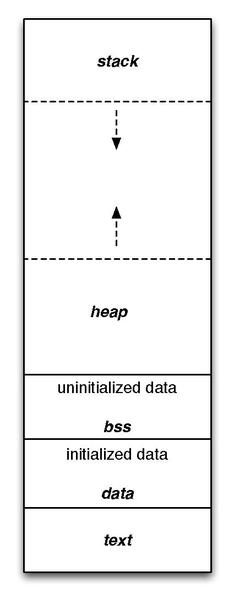
\includegraphics[scale=0.9]{stackHeap.jpg}
\centering
\end{figure}

Durante l'esecuzione un processo può trovarsi in diversi \textit{stati}. 
Gli stati possibili sono:
\begin{itemize}
	\item Nuovo (new): il processo è creato, ma non è ancora ammesso all'esecuzione.
	\item Pronto (ready): il processo può essere eseguito.
	\item In esecuzione (running): le sue instruzioni sono in esezuzione su un processore.
	\item In attesa (waiting): il porcesso non è esecuzione perchè sta aspettando un evento (es. input utente..).
	\item Terminato (terminated): il processo ha terminato l'esecuzione.
\end{itemize}

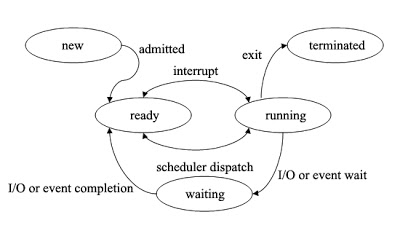
\includegraphics[scale=0.8]{processStateDiagram.jpg}

\subsubsection{Process Control Block}
Detto anche "Task Control Block", contiene le informazioni relative ad un processo:
\begin{itemize}
	\item Process state: ready, running...
	\item Program number (o PID): identifica il processo
	\item Program counter: contenuto del registro "istruzione successiva"
	\item Register: contenuto dei registri del processore
	\item Informazioni di scheduling: priorità, puntatori a code di scheduling..
	\item Informazioni relative alla gestione della memoria: memoria allocata al processo
	\item Informazioni di accounting: CPU utilizzta, tempo trascorso..
	\item Informazioni su I/O: dispositivi asseganti al processo, elenchi file aperti...
\end{itemize}
\begin{figure}[ht]
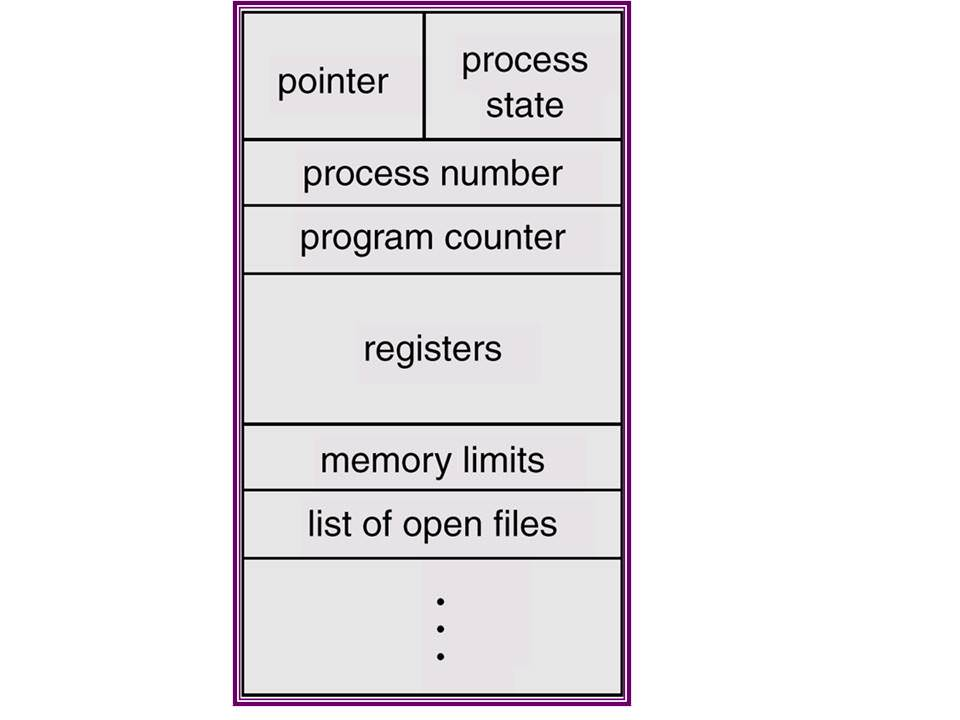
\includegraphics[scale=0.3]{ProcessControl.jpg}
\centering
\end{figure}

\subsubsection{Threads}
Fino ad ora abbiamo assunto che un processo abbia un singolo flusso di esecuzione sequenziale. Supponiamo che si possano avete molti program counter per un singolo processo:
\begin{enumerate}
\item 
\end{enumerate}

\subsubsection{Scheduling dei processi}
L'obiettivo dello scheduling dei processi è quello di massimizzare l'utilizzo della CPU. Una tecnica per fare questo è quella del \emph{Time-sharing}:

Lo scheduler dei processi sceglie il prossimo processo da eseguire tra quelli in stato ready.
Ci sono diverse code di processi:
\begin{itemize}
 \item Ready queue: processi residenti in memoria
\item Wait queue: diverse code per i processi in attesa
\end{itemize}
Durante la loro vita i processi migrano tra una coda e l'altra.
\\ \\
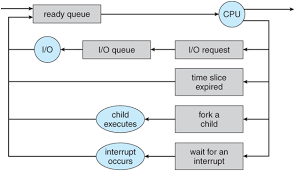
\includegraphics[scale=1.1]{processQueue.png}
\\ \\

Quando un SO decide che si deve cambiare processo, si ha la \textbf{commutazione di contesto} (o \textit{context switch}). Quando la CPU passa ad eseguire un processo diverso, il sistema operativo deve salvare lo stato del processo precedente, e caricare lo stato salvato del processo da rieseguire attaverso un context-switch.
Il PCB rappresenta il contesto di un processo. Il tempo necessario per il context switching è puro overhead: non viene eseguito alcun lavoro utile. Più è complesso l'SO, più è complesso cambiare processo per il context-switch.
\\ \\
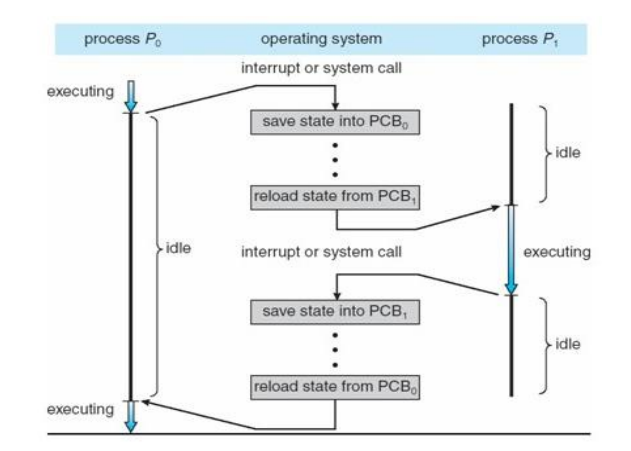
\includegraphics[scale=0.7]{context-switching.png}
\\ \\ 
\paragraph{Multitasking nei sistemi mobili} Alcuni sistemi mobili (es. le prime versioni di iOS) permettevano solo ad un processo di essere in esecuzione. Da iOS4 è possibile avere un processo in esecuzione in \textbf{foreground} (ha lo schermo a disposizione) e un certo numero di processi in esecuzione in \textbf{background} (senza schermo), ma con dei limiti.
Android ha molti meno limiti: i processi in background che vogliono effettuare delle elaborazioni devono creare opportuni \textit{servizi}, che:
\begin{itemize}
\item non hanno interfaccia utente
\item possono usare un ridotto contenuto di memoria
\item possono continuare a funxionare anche quando l'app in backgorund è sospesa
\end{itemize}
L'aumento di potenza dei sistemi mobili rende i loro OS sempre più simili a quelli non mobili.

\subsection{Operazioni sui processi}
\subsubsection{Creazione di processi}
Di solito nei sistemi operativi i processi sono organizzati in maniera gerarchica:
\begin{itemize}
\item un processo (padre) può creare diversi processi (figli) fino a creare un \textit{albero di processi}.
\item PORCODDIO PERCHECAZZO VA COSI VELOCE
\end{itemize}
Sistemi operativi diversi creano processi in modo diverso. Possono esistere diverse politiche di condivisione (padre e figlio condividono le risorse, solo alcune, nessuna), diverse politiche di creazione di spazio di indirizzi (il figlio è un duplicato del padre (stessa memoria e programma, oppure il figlio deve eseguire qualcos'altro) e ancora politiche di coordinazione padre/figli (il padre è sospeso finchè i figli non terminano, oppure eseguono in maniera concorrente).
\end{document}
